O MediaWiki é o território virtual onde os wikipedistas vivem. O sistema de gestão de plataformas wikis, criado e mantido pela própria comunidade Wikimedia, organiza e sistematiza não só as formas como os conteúdos são exibidos como também as dinâmicas de interação e organização das comunidades que o utilizam.

A utilização massiva do MediaWiki é muito cara à comunidade Wikimedia, que não vê com bons olhos a utilização de outras ferramentas de gestão de tarefas ou de comunicação, buscando sempre estimular que a ferramenta seja utilizada para tudo que for possível.

Em seus primórdios, a Wikipédia utilizava outra ferramenta para gestão de suas wikis, o UseModWiki \citep{lih_wikirevolution_2009}. Mas, dado seu crescimento e a demanda por atendimento a uma escala de visitas maior que qualquer outra wiki do planeta, somada a anseios cada vez maiores por customizações do sistema para suas dinâmicas, a comunidade, liderada pelo voluntário Magnus Manske, resolve desenvolver seu próprio sistema gestor de wikis e cria uma comunidade independente dedicada ao desenvolvimento do software.

Desde então, o Movimento Wikimedia estabeleceu diversos outros projetos de criação de conteúdos educacionais, mas até hoje o MediaWiki é o único projeto oficial do Movimento Wikimedia cujo produto final é um software.

A necessidade de habilidades específicas para escrita de código-fonte para o MediaWiki torna este projeto diferente dos demais, onde (nos demais) editores podem transitar com maior facilidade. Considerando que a maioria dos wikimedistas não são programadores, o projeto  MediaWiki acaba criando uma comunidade dentro do movimento Wikimedia mais restrita e menos acessível para participantes de outros projetos.

Não obstante ser um projeto irmão da enciclopédia e ter seu código-fonte aberto, o MediaWiki é estabilizado na operação diária da Wikipédia como uma caixa-preta. Sua atuação cotidiana assim se torna invisível, e somente seus \textit{outputs} são levados em conta. Exatamente como previsto por Bruno Latour, a comunidade somente se atenta para a forma como a caixa-preta funciona em momentos de pane que bloqueem a operação padrão rotineira. Apenas quando se fazem necessários desvios de rota e angariamentos de novas composições que a caixa-preta do MediaWiki é aberta, dissecada, questionada e posta a prova, conforme veremos mais detalhadamente nas próximas seções.

Mesmo os usuários não programadores, apesar de não ``viverem'' o dia-a-dia da comunidade MediaWiki, são agentes que estão sempre negociando com este software a operação diária das Wikipédias. É fácil notar como muitas vezes discussões sobre mudanças de regras passam por questionamentos como ``\textit{dá para fazer isso no MediaWiki?}'' ou ``\textit{algum voluntário programador poderia fazer aquilo?}''. O sistema é um ator ativo na construção da governança das Wikipédias, que muitas vezes se mostra intransigente em seus posicionamentos e delimita fronteiras de atuação. Assim, acaba fornecendo a seus porta-vozes um grande poder, os autorizando a decretar ``inviabilidade técnica'' de determinadas propostas quando oportuno.

Além de sua atuação na negociação de confecção de regras, inúmeras vezes cabe ao MediaWiki ser o papel de ser o responsável por garantir o cumprimento das mesmas. Visando ``ganharem tempo'' para realizar tarefas percebidas como mais nobres ou prazenteiras, wikipedistas delegam para o software várias tarefas ditas óbvias de controle do que pode ser editado na Wikipédia. Na prática, o MediaWiki atua como uma ``barreira de primeiro nível'' extremamente confiável, bloqueando e filtrando edições que ``obviamente'' não deveriam ser salvas, sem ter sua atuação escrutinada corriqueiramente por nenhum outro ator.

Diferente das regras que são fiscalizadas e aplicadas por usuários, sejam humanos ou robôs, que deixam rastros digitais claros em espaços frequentemente visitados pela comunidade (como a página de ``Mudanças Recentes''), as ações tomadas pelo MediaWiki são logadas em espaços mais obscuros de seu banco de dados, conhecidos apenas por um pequeno número de programadores.

Enquanto as demais regras, que estão a todo tempo exibindo os resultados práticos de sua aplicação para os wikipedistas, acabam de tempos em tempos sendo questionadas e rediscutidas, o mesmo raramente acontece com aquelas que estão programadas no MediaWiki.

Acreditamos que, exatamente por estarem implementadas em códigos-fontes automatizados, as regras aplicadas pelo MediaWiki acabam ganhando o status de inquestionáveis, e passam despercebidas mesmo por usuários mais aguerridos em todos os debates ligados a governança do projeto. Afinal, não se pode questionar o que não se vê.

Com isso, podemos falar que o MediaWiki se porta como o grande juiz dos casos invisíveis da Wikipédia. Ou, em outras palavras, que o software atua como uma rede que consolida uma caixa-preta. Entendendo que ``\textit{tem-se uma caixa-preta quando muitos elementos são levados a atuar como um só}'' \citep[205]{latour_ciencia_1987}, e seguindo o interesse desta pesquisa em abrir caixas-pretas, partimos então nas próximas páginas a observar quais elementos configuram esta rede e realizam traduções que permitem sua estabilização.

Assim como todo software gestor de conteúdos, o MediaWiki media as interações e ao mesmo tempo direciona os caminhos dos usuários na plataforma. Dentre as dezenas de atividades performadas por ele, elegemos enquadrar em nossa pesquisa três grupos de funcionalidades que podem explicitar com riqueza esse movimento de tradução de interesses e estabilização de uma caixa-preta, pois atuam diretamente com questões sempre presentes em discussões sobre regras editoriais e tem sua calibragem definida por regras estabelecidas por usuários. São elas: ``lista branca e lista negra'', ``filtros de edição'' e ``CAPTCHA''.

\subsection{Lista Negra e Lista Branca}

Segundo a própria Wikipédia, uma ``lista negra'' é uma lista ``\textit{que, por alguma razão, nega certos direitos, serviços, participação ou mobilidade a alguém ou a alguma entidade, em determinada situação, período de tempo ou lugar}''. \citewiki{ptwiki_lista_negra_definicao}

Ainda segundo a Wikipédia, ``\textit{em informática, usa-se o termo lista negra ( ou Blacklist (em inglês) ) para designar uma lista de e-mails, endereços IP ou até mesmo domínios, que identificam fontes de spam. \textit{Freqüentemente} torna-se útil esse auxílio com o intuito de restringir todos os elementos de uma rede que inspiram desconfiança de spam}''.

Dentro das Wikipédias, as listas negras existem ``\textit{principalmente para controlar o spam generalizado e a perturbação dos projetos da Wikimedia Foundation}''. \citewiki{ptwiki_lista_negra}

Segundo a regra sobre a utilização de ``Ligações externas''\footnote{Não muito utilizada neste contexto no Brasil, a palavra "ligação" aqui significa um \textit{link} para uma página web.} para outros sites, existem três tipos de links que são proibidos na Wikipédia em português: (1) links com códigos de marketing de afiliados, (2) links para conteúdos com violação de direito autoral e (3) ``\textit{websites que façam parte da lista de spam local ou global sem que tenham sido whitelisted}''. Diferente das duas primeiras proibições, esta terceira é complementada com a seguinte afirmação: ``\textbf{\textit{O código MediaWiki bloqueia automaticamente quaisquer edições com essas ligações}}''. \citewiki{ptwiki_ligacoes_externas_ligacoes_proibidas}

Cabe explicar que o termo ``\textit{whitelisted}'' da citação acima deve ser entendido como ``colocado na lista branca''. Lista esta que funciona como uma coletânea de exceções às listas negras. A lista negra então pode ser vista como a lista principal, onde domínios\footnote{Domínio aqui é usado para falar sobre a base dos endereços utilizados para encontrar servidores na internet, e normalmente contêm diversas páginas em suas estruturas. Se traduzido para o inglês, seria utilizada a palavra ``\textit{domain}''. Não confundir com ditos em português ``domínios'' internos da Wikipédia, que em inglês são chamados de ``\textit{namespaces}''.} são bloqueados. Já a lista branca tenderá a conter páginas específicas que podem ser liberadas em domínios indesejados (ou domínios inteiros que se deseje liberar em projeto e estejam bloqueados na lista negra global).

Sempre que uma edição é salva em um projeto Wikimedia, o MediaWiki varre duas listas negras verificando todos os links externos adicionados. Uma lista é mantida pela comunidade local (como a Wikipédia em português), e a outra pela comunidade global. Caso o software encontre o domínio da URL de um dos links adicionados em uma das listas negras, ele então busca por exceções na lista branca local.

Caso não encontre uma exceção que se aplique ao link desejado, é exibido ao usuário um aviso informando que ``\textit{não foi possível salvar (Gravar) a página devido ao bloqueio do filtro de spam}'', com um link para a página com mais informações sobre o ``\textit{filtro de spam da Wikipédia}'' \citewiki{ptwiki_mediawiki_spam_blacklist_info}.

\begin{figure}[H]
    \centering
    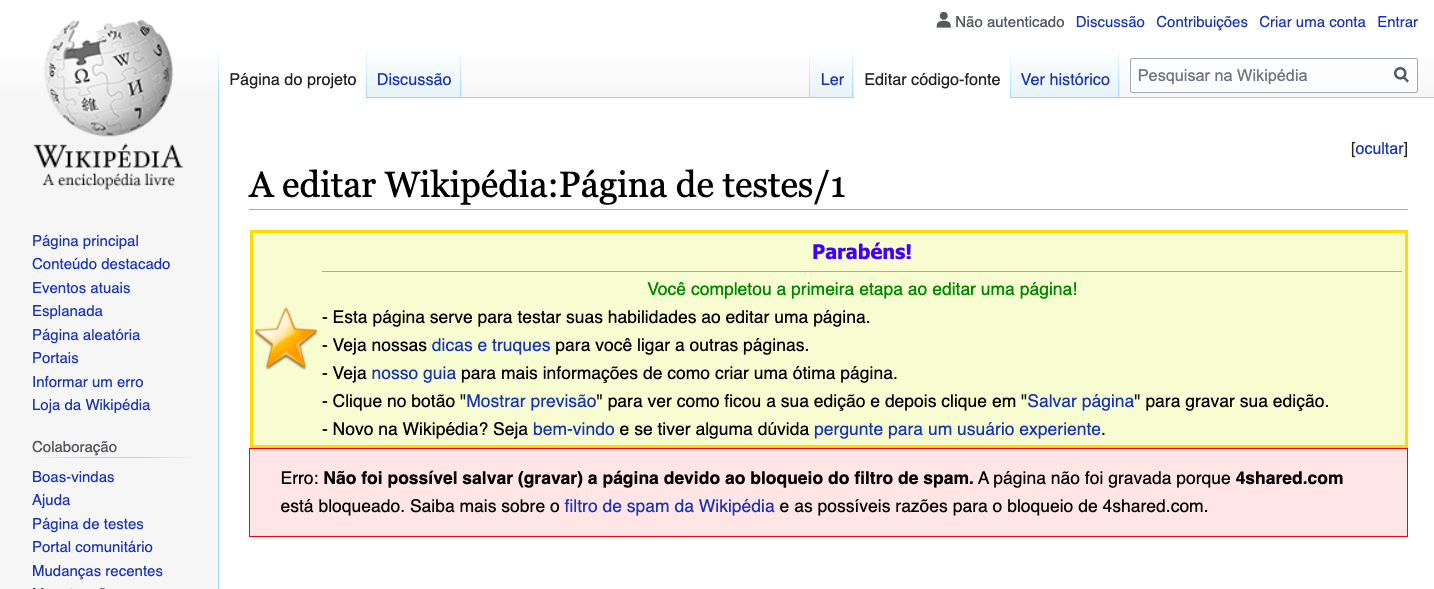
\includegraphics[width=1\textwidth]{Images/mediawiki_blacklist.png}
    \caption{Na caixa vermelha pode ser vista a mensagem que o MediaWiki exibe ao proibir uma edição que adicionaria um link para uma página listada na blacklist.}
    \label{fig:mediawiki_blacklist}
\end{figure}

Ao final desta página, é informado ao usuário que ``\textit{caso você acredite que um endereço não deveria estar bloqueado, é possível solicitar uma exceção para esta página em particular ou o desbloqueio do site}'', com links internos para as páginas onde as solicitações podem ser feitas.

Todas as discussões de bloqueio ou desbloqueio de links devem ser feitas em páginas wikis do projeto local. Buscando organizar suas páginas administrativas, muitas vezes as comunidades criam \textit{templates} que devem ser utilizados em pedidos para padronizar a forma como são apresentados. No caso do link citado no parágrafo anterior, o usuário não somente será encaminhado para a página de discussão da ``Spam-whitelist'', como o bloco de edição já aparecerá preenchido com o \textit{template}, conforme pode ser visto na figura:

\begin{figure}[H]
    \centering
    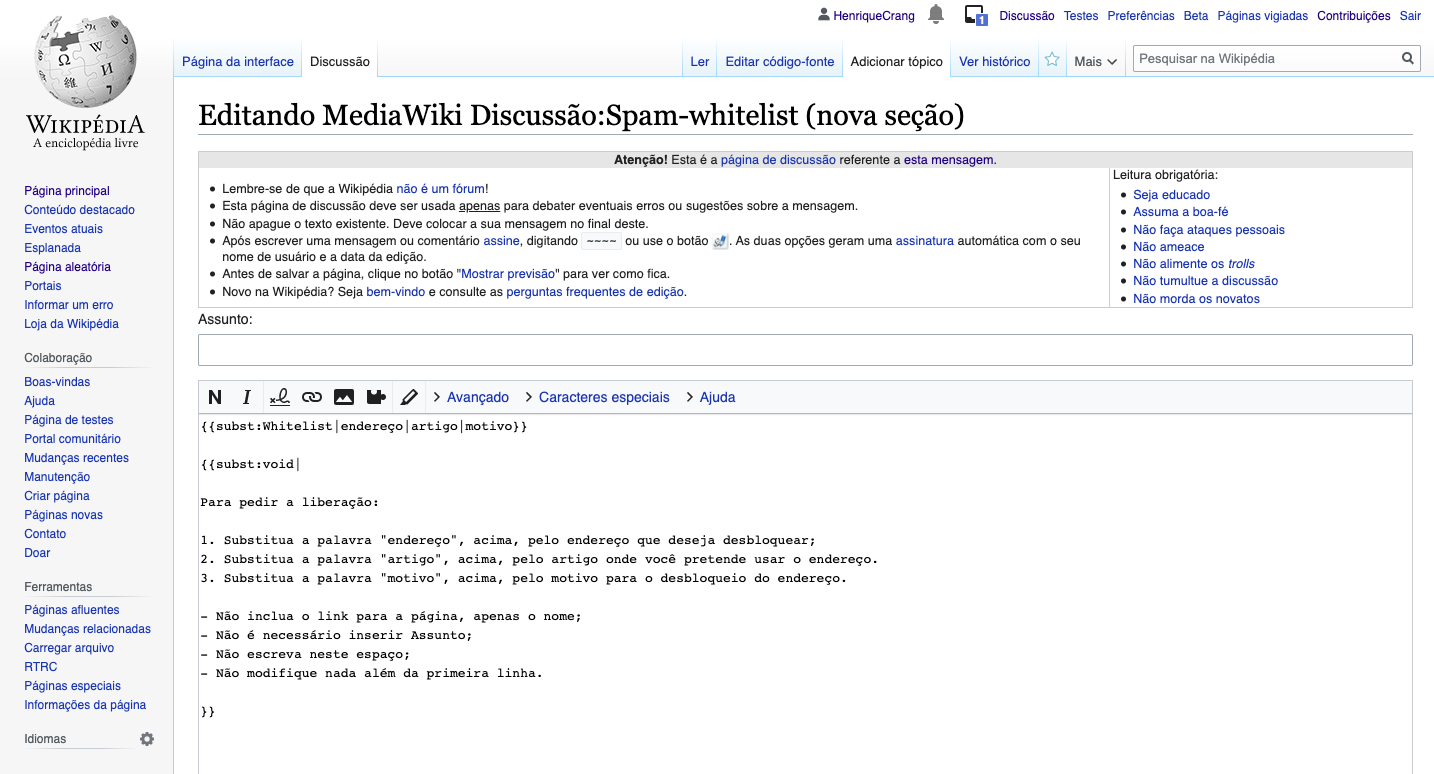
\includegraphics[width=1\textwidth]{Images/mediawiki_spam_whitelist.png}
    \caption{Página que é exibida quando um usuário clica no link interno para solicitar uma exceção à lista negra.}
    \label{fig:mediawiki_spam_whitelist}
\end{figure}

Essa estrutura de \textit{templates} é muito conhecida pela comunidade e sua utilização é fluida para wikipedistas experientes, mas é comum usuários novatos não entenderem as instruções ali contidas e preencherem o \textit{template} nos locais errados e/ou não desenvolverem no espaço reservado para o ``motivo'' da solicitação os argumentos esperados pelos wikipedistas, levando a diversos pedidos serem negados sem que pudessem ser devidamente compreendidos. \citewiki{ptwiki_mediawiki_discussao_spam_whitelist}

Além do uso do template, também não é trivial para editores recém chegados a diferença entre ``pedir para um endereço ser adicionado à whitelist'' e ``pedir para um endereço ser removido da blacklist''. Como dito pelo administrador Edmond Dantès em resposta a um pedido de exceção na lista branca, ``\textit{Não liberamos domínios}'' \citewiki{ptwiki_mediawiki_discussao_spam_whitelist}. Caso um usuário deseje retirar um domínio inteiro da lista negra, a comunidade espera que ele se dirija a outro local: a página de discussão ``MediaWiki:Spam-blacklist'' \citewiki{ptwiki_mediawiki_discussao_spam_blacklist}.

Esta página ``MediaWiki:Spam-blacklist'', onde fica a lista de sites bloqueados, já foi editada 3275 vezes, enquanto a página ``MediaWiki:Spam-whitelist'', onde o MediaWiki encontra a lista de exceções,  apresenta 276 alterações. (\cite{quarry_edit_mediawiki_namespace}). Já suas respectivas páginas de discussão, onde os pedidos são feitos, não apresentam a mesma desproporção. 2347 edições foram feitas na página com pedidos de adição de sites na lista negra, enquanto 3208 edições foram realizadas na discussão sobre a lista branca (\cite{quarry_edit_mediawiki_talk_namespace}). Essa grande diferença na proporção entre edições na página de discussão e na página principal sugere que boa parte dos pedidos de bloqueio feitos são implementados, enquanto a maioria dos pedidos de exceções são negados.

Todas as edições na página de discussão da \textit{blacklist} foram feitas por apenas 166 usuários, sendo que só 37 deles fizeram mais de dez edições cada. (\cite{quarry_edit_sbl_talk_page}) Já nas discussões de exceções, encontramos a participação de 659 usuários distintos (\cite{quarry_edit_swl_talk_page}), mas com um número ainda menor de usuários fazendo mais que dez edições: 27.

Esses números sugerem que a discussão sobre \textit{blacklist} tende a ser mais concentrada, com usuários experientes que a conhecem debatendo quais sites devem ser bloqueados, enquanto a lista branca (talvez inclusive por ser linkada na mensagem de bloqueio conforme visto na figura anterior), atrai um número maior de usuários não tão engajados em a acompanhar, provavelmente interessados apenas em seu pedido específico.

Seguindo o rastro desta hipótese, encontramos 380 usuários com uma única edição na discussão da whitelist (\cite{quarry_only_1edit_swl_talk_page}), enquanto sua contraparte negra conta apenas com 44 editores nesta situação (\cite{quarry_only_1edit_sbl_talk_page}). Esses números claramente demonstram que as páginas tem dinâmicas de participação bem distintas, com usuários não engajados na confecção das regras claramente mais preocupados em tentar liberar determinado tipo de edição do que em proibir.

Após todas essas edições, hoje a \textit{Blacklist} da Wikipédia em português apresenta mais de 3000 domínios proibidos de serem linkados, que se somam as mais de 11 mil entradas na lista de Spam Global do Movimento Wikimedia \citewiki{enwiki_wikimedia_spam_blacklist}. Cabe destacar que muitas destas entradas são feitas utilizando expressões regulares \footnote{Expressões regulares, ou \textit{regex}, são uma forma de representar cadeias de caracteres que devam ser identificados por uma determinada função.} que podem bloquear diversos domínios de uma vez, tornando impossível precisarmos o número total de domínios proibidos. Já a lista de exceções da Wikipédia em português apresenta um tamanho muito mais humilde, com 117 endereços especificados.

\subsubsection{Deslocamentos e aumento de escopo}

Apesar de criadas para combater a ação de \textit{spammers}, com o passar do tempo a comunidade passou a delegar também às listas negras do MediaWiki a tarefa de impedir edições que adicionem links para domínios que sejam considerados inapropriados como referências para os verbetes, como hoje pode ser lido na própria página com mais informações sobre o funcionamento da Spam-blacklist: ``\textit{Por decisão da comunidade, alguns sites são considerados fontes não-confiáveis e são bloqueados para evitar sua utilização em artigos}'' \citewiki{ptwiki_mediawiki_spam_blacklist_info}.

Esta nova utilidade da ferramenta não se estabilizou sem controvérsias. Como podemos observar em uma discussão acontecida na Esplanada \footnote{A Esplanada é uma página interna da Wikipédia em português que funciona como um fórum geral, onde editores podem compartilhar e debater notícias, ideias e propostas.} em 2012 \citewiki{ptwiki_esplanada_geral_spam_blacklist}, quando o usuário Braswiki chamou a atenção da comunidade para a prática que estava se tornando habitual e perguntou: ``\textit{a lista negra de spam deve servir para impedir a inclusão de fontes não fiáveis ou apenas se esses sites estiverem sendo utilizadas como spam?}''

Nesta discussão encontramos a fala do usuário Desempates, que demonstra preocupação com o uso ``deturpado'' da ferramenta que deveria coibir spam: ``\textit{Um problema que noto é que está havendo uma deturpação dos objetivos originais da lista. Como o próprio nome indica, uma Spam-blacklist, visaria exclusivamente o bloqueio de sites de spammers. Para os demais casos, como a falta de fiabilidade, seria mais adequado que houvesse uma outra listagem}''. Sua fala é reforçada pela posição de Helder, que comenta ``\textit{a MediaWiki:Spam-blacklist deve ser usada para impedir SPAM, isto é, propaganda \textbf{em massa}, não propagandas em circunstâncias isoladas, como as feitas por um único editor ou em um único artigo, muito menos para fazer  ‘controle de qualidade’ das ligações externas.}'' (grifo do original), destacando ainda em seu posicionamento os resultados de uma pesquisa realizada pela WMF em 2011, que apontava para o volume de edições na blacklist lusófona ser maior que o dobro das listas francófona e espanófana. \citewiki{enwiki_wikimedia_research_talk}.

O debate segue com usuários defendendo que a prática de adicionar um site na blacklist não seja burocratizada, e que administradores continuem tendo a liberdade de realizar esta inclusão sem depender de uma consulta prévia a comunidade. Tal situação desperta preocupação ao usuário Desempates, que nota ``\textit{estar havendo uma deturpação dos objetivos da Spam-blacklist. Alguns administradores se apropiaram (sic) dela para utilizá-la como ferramenta de censura, bloqueando websites dos quais discordam, alegando uma suposta não-fiabilidade das fontes}''.

Buscando uma solução pacificadora, Helder começa a rascunhar uma proposta intermediária, utilizando outra ferramenta do MediaWiki, mas que esbarraria em problemas de performance do software: ``\textit{Talvez o uso de um filtro para lidar com as  ‘excessões’ seja uma boa ideia. Uma das vantagens é que cada filtro pode exibir um aviso personalizado explicando o motivo pelo qual a edição foi barrada. Mas também não daria muito certo ter que criar um filtro para cada site (só para explicar o motivo específico daquele site não ser aceito), pois um numero excessivo de filtros prejudicaria a performance do site...}''

A proposta de Helder traria uma diferenciação importante para a experiência dos usuários que tentam adicionar um link na Wikipédia: avisos personalizados. Da forma como estava sendo utilizada a ferramenta até então, um editor que adicionasse um link para uma fonte considerada não-fiável recebia o mesmo aviso de SPAM visto na figura acima.

Porém, a proposta não atrai muita atenção, e a discussão então se alonga para detalhes sobre como um usuário poderia questionar a adição de um endereço na \textit{blacklist}. A comunidade decide então criar uma página chamada ``Central de confiabilidade'', onde ``\textit{Editores podem questionar aqui se fontes são fiáveis em um contexto específico}''. \citewiki{ptwiki_fontes_confiaveis_central_confiabilidade}

O desfecho parece agradar a maioria dos usuários, e o debate original se esvazia. Porém, como observa o usuário Rjclaudio sobre a decisão tomada: ``\textit{não se falou nada sobre a spamblacklist e seu uso como meio de controlar a qualidade das referências / ligações externas para além do impedimento de spam em massa}''. Dentro deste cenário de incertezas, Raimundo75br responde que ``\textit{Parece-me que a partir da discussão na Wikipédia:Fontes fiáveis/Central de fiabilidade pode-se incluir um site na spamblacklist, de modo que tal inclusão seja baseada em uma discussão}'', e o assunto aparenta cair em esquecimento.

Nos dias atuais, conforme pode ser notado na supracitada informação da página de informações sobre a \textit{spam-blacklist}, páginas consideradas não fiáveis continuam podendo ser adicionadas diretamente na lista negra por um administrador, e o usuário que intentar adicionar um link para elas continua recebendo o aviso de que está praticando \textit{spam}. Os pedidos de adição de novas páginas na lista negra por serem fontes não fiáveis seguem podendo ser feitos na página de discussão que levam o termo \textit{spam} em seu nome. Página esta que, como observamos, é acompanhada por um número irrisório de usuários.

\subsection{Filtros de Edição}

Na seção anterior vimos o usuário Helder mencionando a ferramenta de ``filtros de edição'', a apontando como uma possível alternativa para impedir a adição de links para fontes não fiáveis. Sua proposta acabou sendo readaptada e implementada em um interessante caso de um filtro que atua com links para um famoso domínio específico. Mas, antes de detalharmos este caso, devemos compreender melhor o funcionamento da ferramenta de filtros de edição do MediaWiki.

A ferramenta, conhecida originalmente como ``\textit{Abuse Filter}'', foi ativada na Wikipédia em inglês em março de 2009, conforme noticiado pela edição do \textit{The Signpost} do mesmo mês.
 \footnote{``\textit{It was first enabled on English Wikipedia on March 2009}''. \citewiki{enwiki_signpost_abuse_filter}}

Logo no mês seguinte, mais precisamente no dia 16/04/2009, \cite{extension_abuse_filter} a ferramenta é ativada na Wikipédia em português, com seu nome traduzido literalmente para ``filtro de abusos''. Nome este que seria alterado para ``filtro de edições'' pouco tempo depois, em 25/06/2009, mais precisamente às 15h36, \citewiki{ptwiki_filtro_de_edicoes_lechatjaune} 1 hora e 34 minutos após o usuário Lechatjaune ter feito esta proposta na página de discussão e ter recebido o apoio de dois outros usuários. 

Lechatjaune estava preocupado com o fato de haver ``\textit{alguns falsos positivos e o filtro gerar registros visíveis}'' e como isso poderia ofender alguns usuários por serem apontados pelo MediaWiki como ``\textit{abusadores}''. Em seu comentário de apoio, o usuário Daimore pontua que ``\textit{filtro de edições define bem o que acontece e, \textbf{se algum dia o filtro funcionar perfeitamente}, pode ser descrito como \textbf{filtro de edições abusivas} sem problema nenhum}''. (grifos do autor) 

É difícil saber o que se enquadraria dentro da ideia de ``funcionar perfeitamente'' apontada por Daimore. Mas, atualmente podemos observar que o Filtro de edições é uma ferramenta estabilizada e altamente ativa na comunidade lusófona, porém seu nome permanece inalterado até então. \footnote{Fugiria do escopo desta pesquisa investigar o quanto a diferença de nome da ferramenta em diferentes Wikipédias pode influenciar o comportamento de usuários, mas deixamos esta porta aberta para possíveis futuros trabalhos.}

Hoje, segundo sua própria página, o filtro de edições ``\textit{permite implementar regras específicas de controle sobre as edições na Wikipédia e decisões automáticas para certos tipos de situação}'' \citewiki{ptwiki_filtro_de_edicoes}. Na prática, isso significa que sempre que um usuário clica no botão salvar, o MediaWiki observa todos os filtros para saber se algum deles se aplica ao que está sendo salvo. E, em caso da edição der positivo para algum filtro, este pode ordenar quatro diferentes ações ao MediaWiki: ``corresponder'', ``etiquetar'', ``avisar" ou ``desautorizar''.

A ação de ``corresponder'' é a mais branda, e costuma ser utilizada em filtros que estão sendo testados. As edições ``correspondidas'' serão listadas nas páginas específicas de cada filtro, onde usuários que estejam estudando os filtros poderão observar quais edições estão de fato sendo abarcadas pelos critérios do referido filtro e com isso avaliar, por exemplo, seus índices de falsos positivos.

``Etiquetar'', assim como ``corresponder'', é uma ação invisível para o usuário que estiver clicando em salvar. A edição será salva e exibida normalmente na Wikipédia, sem qualquer alteração de rota no fluxo do usuário. Porém, no caso da ``etiquetagem'', o sumário da edição exibirá a etiqueta \footnote{Também conhecidas pelo termo em inglês \textit{tag}.} relativa ao respectivo filtro. Esta etiqueta é exibida em locais muito mais visíveis da Wikipédia do que as páginas dos filtros, como nos históricos de edições e nas páginas de monitoramento de mudanças recentes. Desta forma, as etiquetas são utilizadas para alertar revisores para determinados padrões de edição, podendo ensejar uma ação humana posterior à marcação do filtro.

\begin{figure}[H]
    \centering
    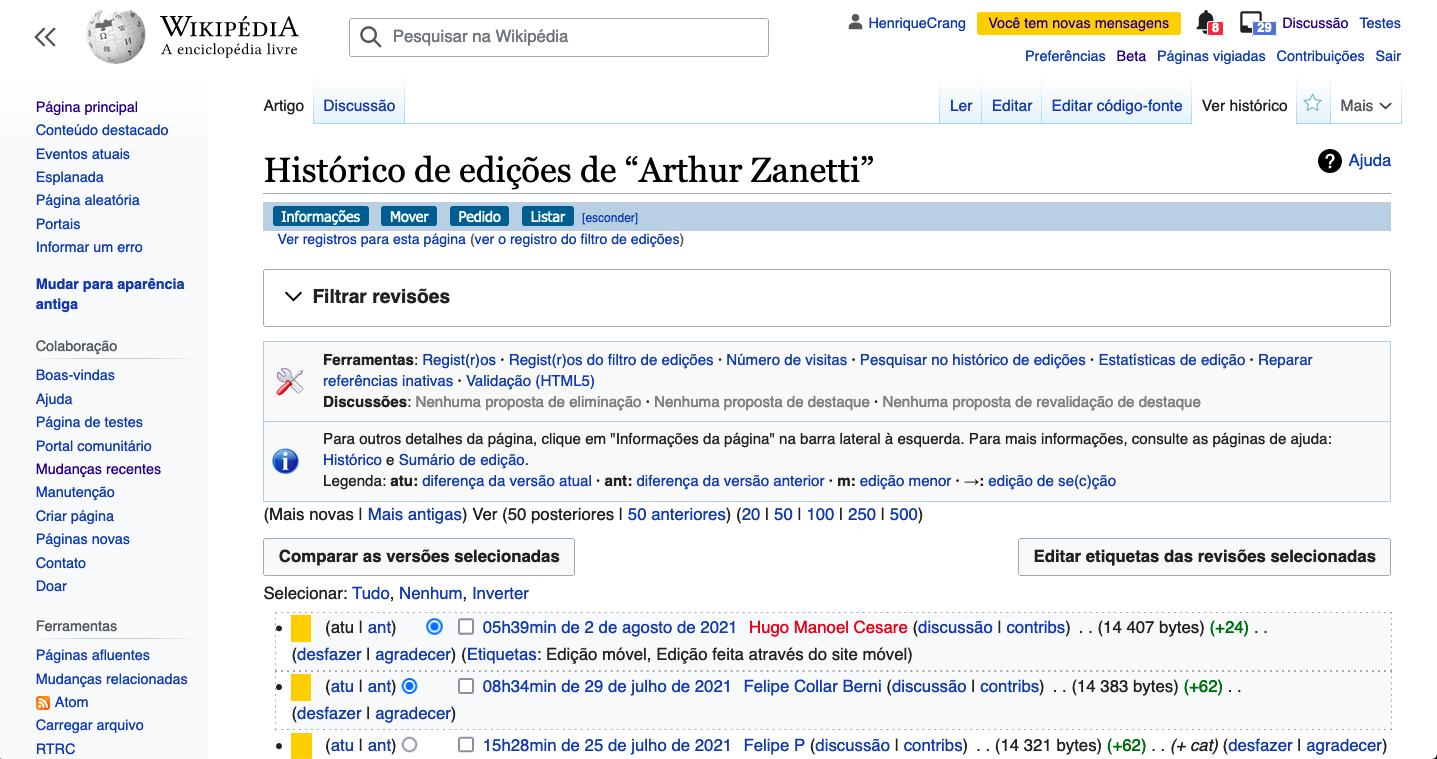
\includegraphics[width=1\textwidth]{Images/mediawiki_etiqueta.png}
    \caption{Exemplo do histórico de edições de uma página, com a edição mais recente recebendo duas etiquetas.}
    \label{fig:mediawiki_etiqueta}
\end{figure}

``Avisar'' já é uma ação que o filtro de edições toma que se faz imediatamente visível ao usuário, e altera sua experiência de edição no MediaWiki. Ao tentar salvar uma edição que algum dos filtros diga que deva ser ``avisada'', ao usuário será apresentada a seguinte mensagem:

\begin{figure}[H]
    \centering
    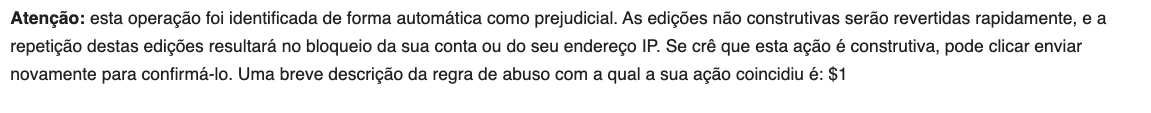
\includegraphics[width=1\textwidth]{Images/mediawiki_avisar.png}
    \caption{Mensagem padrão da função ``avisar'' do Filtro de edição. Para cada caso o ``\$1'' é substituído por uma mensagem do respectivo filtro despelotado. \citewiki{ptwiki_mediawiki_abusefilter_warning}}
    \label{fig:mediawiki_avisar}
\end{figure}

Após ser convidado a refletir se sua edição é ``construtiva'', o usuário tem então a opção de clicar novamente no botão de salvar e, nesta sua segunda tentativa, o MediaWiki deixará o conteúdo ser salvo.

Já a função de ``desautorizar'' é a mais drástica. Uma edição que se enquadre nos critérios de um filtro que preveja uma desautorização não poderá ser salva, e o MediaWiki apresentará ao usuário a seguinte mensagem:

\begin{figure}[H]
    \centering
    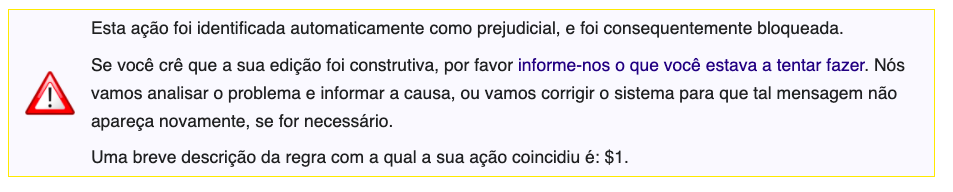
\includegraphics[width=1\textwidth]{Images/mediawiki_desautorizar.png}
    \caption{Mensagem padrão da função ``desautorizar'' do Filtro de edição. Para cada caso o ``\$1'' é substituído por uma mensagem do respectivo filtro despelotado.\citewiki{ptwiki_mediawiki_abusefilter_disallowed}}
    \label{fig:mediawiki_desautorizar}
\end{figure}

Desta forma, quando são utilizadas as ações ``avisar'' e ``desautorizar'' do filtro de edições, estão sendo tomadas decisões prévias sobre o que pode ser salvo. Estas decisões a \textit{priori}, tomadas e executadas de forma automática pelo MediaWiki, acontecem antes dos conteúdos chegarem aos espaços mais visíveis da Wikipédia, onde habitualmente acontecem discussões sobre a pertinência dos conteúdos.

%até aqui está explicando por alto como funcionam os filtros, agora começo a dar contexto pra eles. talvez quebrar seção?

Assim como acontece com a \textit{spam-blacklist}, os filtros também existem tanto em nível local nos projetos como a nível global para todas as wikis do movimento Wikimedia. Por padrão, os filtros globais são aplicados a todas as wiki consideradas de tamanho ``pequeno'' e ``médio'', e às wikis de grande porte que solicitarem sua inclusão. \footnote{``Global abuse filters were subsequently implemented and are set and operated from Meta-Wiki. These global filters apply to small[3] and medium[4] public WMF wikis, and those large wikis that opt-in.[5]. The stewards and meta administrators are able to set global abuse filters.[6]'' https://meta.wikimedia.org/wiki/AbuseFilter}

Desde de julho de 2016, a Wikipédia em português é umas das Wikipédias consideradas grandes que solicitaram sua ativação. A proposta de habilitar os filtros globais por lá foi feita pelo usuário He7d3r \footnote{He7d3r e o já citado Hélder são nomes diferentes utilizados ao longo do tempo pelo mesmo usuário.} no dia 02 de julho e, após receber o apoio de 13 editores fora aprovada sem nenhuma objeção. \citewiki{ptwiki_esplanada_proposta_filtros}. No dia 14/07 o pedido de alteração de configuração foi aberto no Phabricator \footnote{Sistema utilizado pelas comunidades técnicas para gerenciar tarefas. Falaremos mais sobre elas próxima seção.} e,  já em 18/07, dezesseis dias após a proposta ter sido feita e com a interação de 14 usuários, o Stashbot informava que a nova configuração, que dali para frente alteraria bastante a forma como usuários editam a enciclopédia, fora colocada em produção. (\cite{enable_global_abusefilters_ptwiki}).

Hoje, dentre as ditas grandes Wikipédias, além da versão em português, apenas as em francês e em cebuano também utilizam os filtros globais. \footnote{ Para encontrar está informação deve-se buscar no arquivo \textit{InitialiseSettings} da \textit{wikifarm} Wikimedia o seguinte comentário \textit{" // Enabled for all wikis that open, global and small/medium in size"}. O arquivo está disponível em  :https://noc.wikimedia.org/conf/InitialiseSettings.php.txt )}

%aqui parece haver uma mini quebra de seção tb. falei antes da instalacao, agora falo do estado da arte 

Atualmente existem 69 filtros globais ativos, sendo que a grande maioria trabalha buscando padrões de vandalismo \citewiki{enwiki_wikimedia_abuse_filter_management}. Na Wikipédia em português o mais ativo é o filtro global 206, que nos últimos 30 dias foi disparado 4611 vezes, correspondendo a edições que adicionavam links externos feitas por usuários com menos de duas edições. \citewiki{enwiki_editing_abuse_filter_206} Dentre os filtros globais que desautorizam edições, os mais ativos na enciclopédia lusófona são o 72, o 222 e o 240, com respectivamente 55, 28 e 24 edições desautorizadas nos últimos 30 dias \citewiki{ptwiki_acoes_filtros}.

Enquanto o filtro 222 pode ter seu funcionamento auditado por qualquer um, com seu código-fonte responsável por identificar a criação de páginas novas em branco por usuários novatos \citewiki{metawiki_editing_abuse_filter_222} visível para qualquer um que saiba navegar até sua página, os filtros 240 \citewiki{enwiki_editing_abuse_filter_240}e 72 tem seus códigos ocultados \citewiki{enwiki_editing_abuse_filter_72}, e deles podemos apenas ter acesso aos nomes: `\textit{Cannabis/CBD spam}' e `\textit{Global ``ntsamr''-pattern spambot filter}', mas sem podermos observar o código fonte dos mesmos.

\begin{figure}[H]
    \centering
    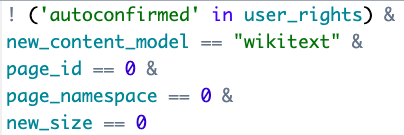
\includegraphics[width=1\textwidth]{Images/codigo_fonte_global_222.png}
    \caption{Código-fonte do filtro global 222. \citewiki{metawiki_editing_abuse_filter_222}}
    \label{fig:codigo_fonte_global_222}
\end{figure}

Tanto os filtros globais como os locais podem ser ``públicos'' ou ``privados''. Um filtro considerado ``público'' é o padrão, onde todas as regras e códigos executados por ele estão publicizados e abertos para receber críticas, comentários e melhorias de toda a comunidade. Já os filtros ``privados'' se valem da chamada ``segurança por obscuridade''. Costumam conter códigos para freiar spams que ``poderiam ser facilmente burlados se o atacante conhecesse a regra'', e então por isso tem seu código fonte aberto apenas para administradores.

De todos os 69 filtros globais atualmente ativos, 18 são ``públicos'' e 51 ``privados''. Quando ocorreu a aprovação da utilização dos filtros globais na Wikipédia em português, nenhum dos 13 editores que participaram do diálogo se preocuparam em ter algum tipo de acesso ao código fonte destes filtros globais fechados, que foram aprovados como confiáveis caixas pretas. \citewiki{enwiki_abuse_filter_management_100_pages}

\begin{figure}[H]
    \centering
    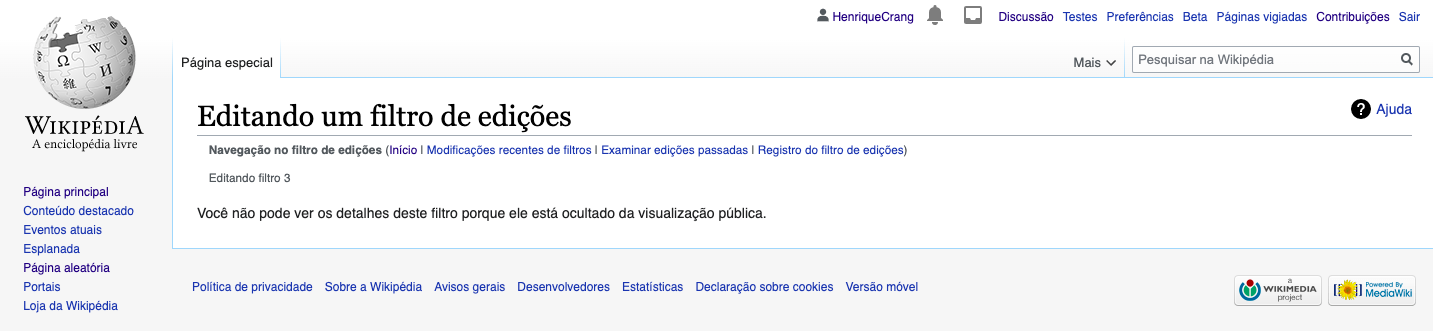
\includegraphics[width=1\textwidth]{Images/pagina_filtro_privado.png}
    \caption{Página especial de um filtro privado \citewiki{ptwiki_pagina_filtro_privado}.}
    \label{fig:pagina_filtro_privado}
\end{figure}

%dei aqui uma geral em filtros globais e seu impacto local. talvez possa trazer para cá umas coisas que já tenho rascunhadas sobre local/global

% agora vou entrar em mais detalhes da criação de filtros na ptwiki

Já dentre os filtros locais, criados pela própria comunidade da Wikipédia em português, os principais com a função de ``desautorizar'' são públicos. Os filtros 113, 18 e 70, com mais de 250 mil edições desautorizadas cada, podem ter seus códigos sobre \textit{"Página nova possivelmente sem referências"}, \textit{"Conteúdo e/ou resumo indevido"} e \textit{"Conteúdo e/ou resumo indevido relacionado ao corpo humano"} amplamente escrutinados pela comunidade. Já os três mais ativos filtros que ``avisam''; 3, 139 e 112, são privados, e por essa característica nossa pesquisa não pode ter acesso direto, através da página de filtros do MediaWiki, ao seu número de ações realizadas.

Porém, driblando de alguma forma a obscuridade de informações pelas páginas do MediaWiki, percebemos que ao ordenar os filtros por sua \textit{``contagem de correspondências''}, conseguimos ter uma ideia da escala da atividade dos filtros privados. Conforme pode ser visto na próxima figura, o filtro 03, sobre \textit{``Remoção considerável de conteúdo''} é o mais ativo na Wikipédia lusófona, com mais ações que o segundo colocado, que apresenta publicamente aproximadamente 267 mil ações.

\begin{figure}[H]
    \centering
    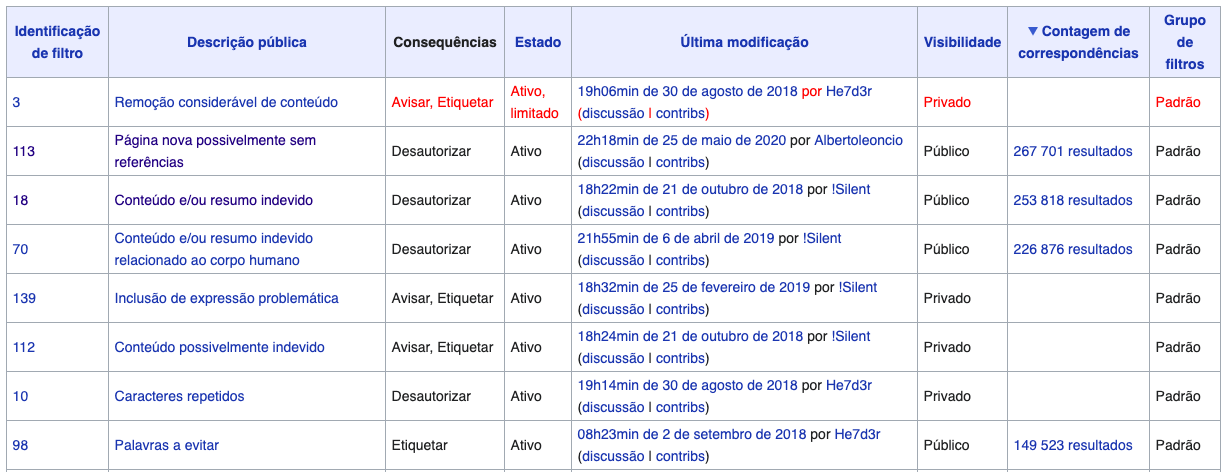
\includegraphics[width=1\textwidth]{Images/historico_filtros_wikipedia.png}
    \caption{Histórico dos filtros da Wikipédia em português ordenados por ``Contagem de correspondências'' \citewiki{ptwiki_administracao_filtros_abusos_100}}
    \label{fig:historico_filtros_wikipedia}
\end{figure}

Já os filtros 139, sobre \textit{``Inclusão de expressão problemática''} e 112 para \textit{``Conteúdo possivelmente indevido''}, com seus nomes um tanto quanto vagos e códigos ocultos, aparecem com um volume de ações menor que 226 mil, mas superior a 149.523. \citewiki{ptwiki_administracao_filtros_abusos_100}

Avançando com nossa pesquisa, resolvemos ir além das páginas da interface do MediaWiki e, consultando os bancos de dados públicos da Wikipédia em português, descobrimos que os quantitativos precisos de ações performadas por cada filtro privado está disponível sim para todos (todos que saibam SQL e conheçam a estrutura do banco de dados do MediaWiki). Lá, no acesso direto aos bancos de dados, então descobrimos que o filtro 139 foi disparado mais de 177 mil vezes, enquanto o 112 está quase empatado com 176 mil avisos feitos. Se esses dois filtros estão dentro do quantitativo previsto, e seus números precisos não agregam mais que uma curiosidade à nossa pesquisa, o mesmo não pode ser dito sobre o filtro 03. 

Sobre o filtro mais ativo da Wikipédia em português, através das páginas públicas, sabíamos apenas que possuía mais disparos que o segundo colocado, que apresenta aproximadamente 267 mil ações, mas não tínhamos ideia da grandeza de sua liderança. Ao consultar o banco de dados, pudemos encontrar incríveis 654.358 edições ``avisadas'' e ``etiquetadas'' pelo privado filtro de ``Remoção considerável de conteúdo'', representando 144\% mais ações que o filtro que aparece em segundo lugar.

\begin{figure}[H]
    \centering
    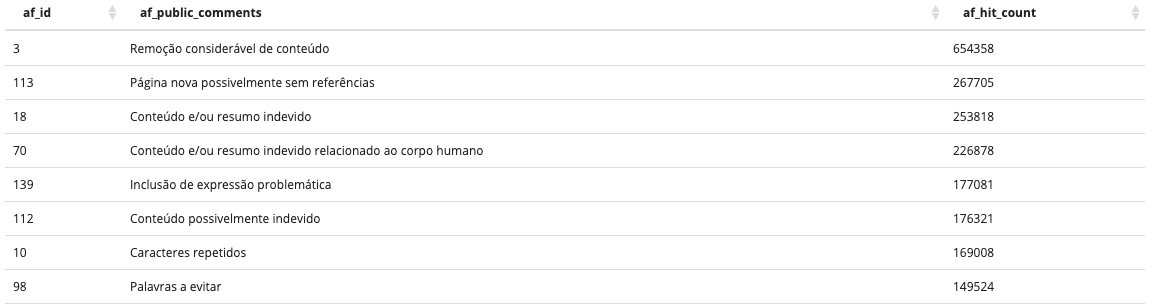
\includegraphics[width=1\textwidth]{Images/mediawiki_bancos_dados_publicos.png}
    \caption{Total de ações realizadas por cada filtro de edições da Wikipédia em português. Dados a princípio não disponíveis pela interface navegável do MediaWiki estão consolidados em bancos de dados públicos.
(\cite{quarry_most_hit_filters})}
    \label{fig:mediawiki_bancos_dados_publicos}
\end{figure}

Ao total, os filtros na Wikipédia em português já foram disparados 5.529.707 vezes (\cite{quarry_filters_count}). Destas, 2.444.513, ou 44\%, foram ações de ``avisos'', enquanto 2.149.290, ou 38,8\%, foram ações que desautorizaram uma edição. (\cite{quarry_warn_disallow_filter_actions}). Dentre todas essas ações que alteram o curso dos usuários, 1.581.419, ou 34,4\%, foram realizadas por filtros ``privados''. (\cite{quarry_warn_disallow_filter_actions_visibility})

Esse massivo volume de edições que tem seu curso esperado bloqueado pelo MediaWiki, através da configuração do filtro de edições, nos mostra que, enquanto alguns usuários devotam grande energia em discussões sobre eliminações e reversões de páginas avulsas, os poucos usuários que controlam os códigos fontes dos filtros atuam em uma escala muito maior. E esta ação em escala costuma passar despercebida pela comunidade, pois suas regras implementadas em códigos privados viram a lei que decide previamente não somente quais edições poderão ser salvas, mas também quais edições poderão ter sua validade debatidas, limitando quais que terão o privilégio de chegar aos espaços de escrutínio visíveis pela ampla comunidade.

\textbf{Como são criados os filtros de edições}

Sabendo de tamanha importância dos filtros de edições na Wikipédia buscamos então entender como eles são criados e editados. Assim como praticamente tudo que acontece no movimento Wikimedia, os filtros de edição são organizados através de páginas wiki. Porém, suas páginas seguem um padrão distinto do usual. Para cada filtro existe uma página ``Especial'', funcionalidade do MediaWiki que permite criar páginas com estruturas pré-prontas e com áreas pré-direcionadas de edição permitida, diferente das páginas padrão que podem ser inteiramente editadas.

\begin{figure}[H]
    \centering
    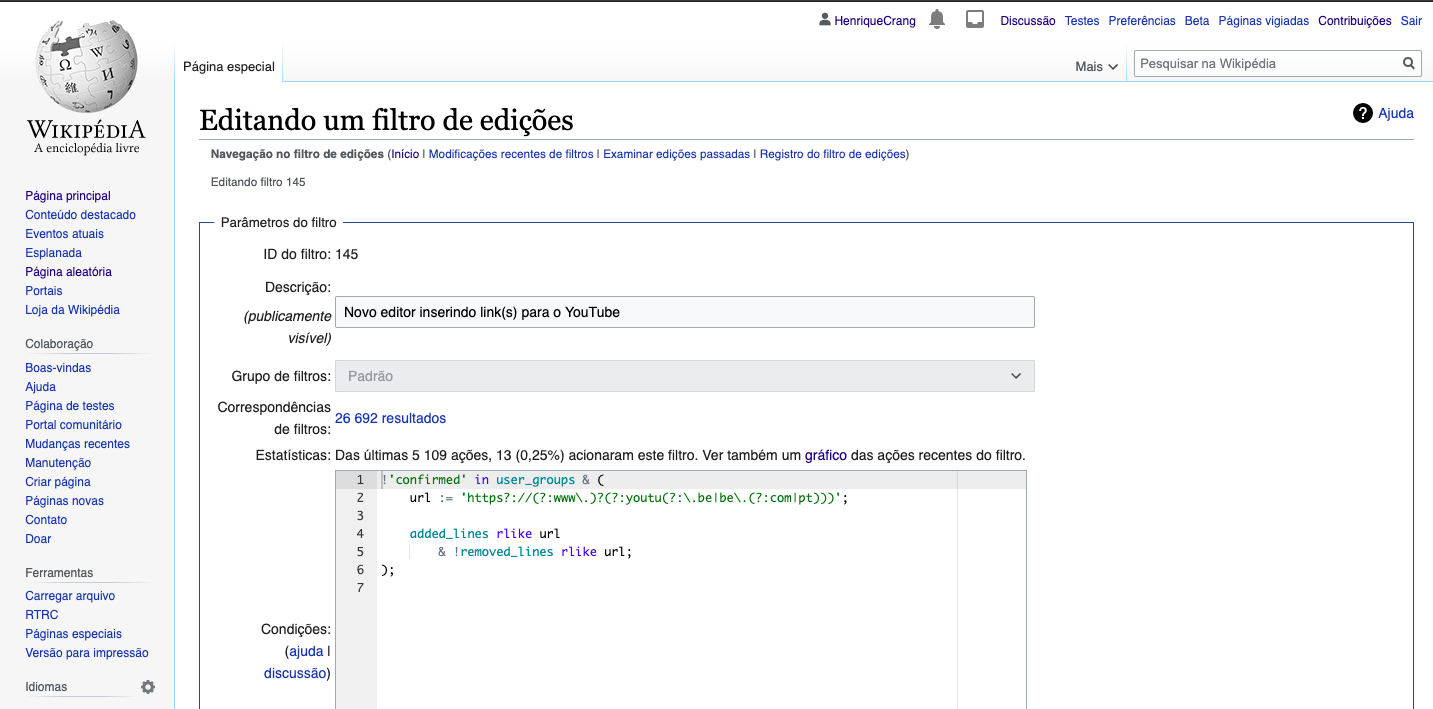
\includegraphics[width=1\textwidth]{Images/pagina_filtro_edicao.png}
    \caption{Exemplo de uma página especial relativa a um filtro de edição \citewiki{ptwiki_editar_filtros_edicao}.}
    \label{fig:pagina_filtro_edicao}
\end{figure}

Nestas páginas especiais, usuários administradores podem, para cada filtro, editar as expressões regulares, ativá-lo ou desativá-lo, configurar quais ações serão tomadas por ele, editar a mensagem que será exibida para o usuário que for identificado pelo filtro e deixar notas sobre seu trabalho realizado no filtro para auxiliar o trabalho de voluntários que venham a editá-lo no futuro.

\begin{figure}[H]
    \centering
    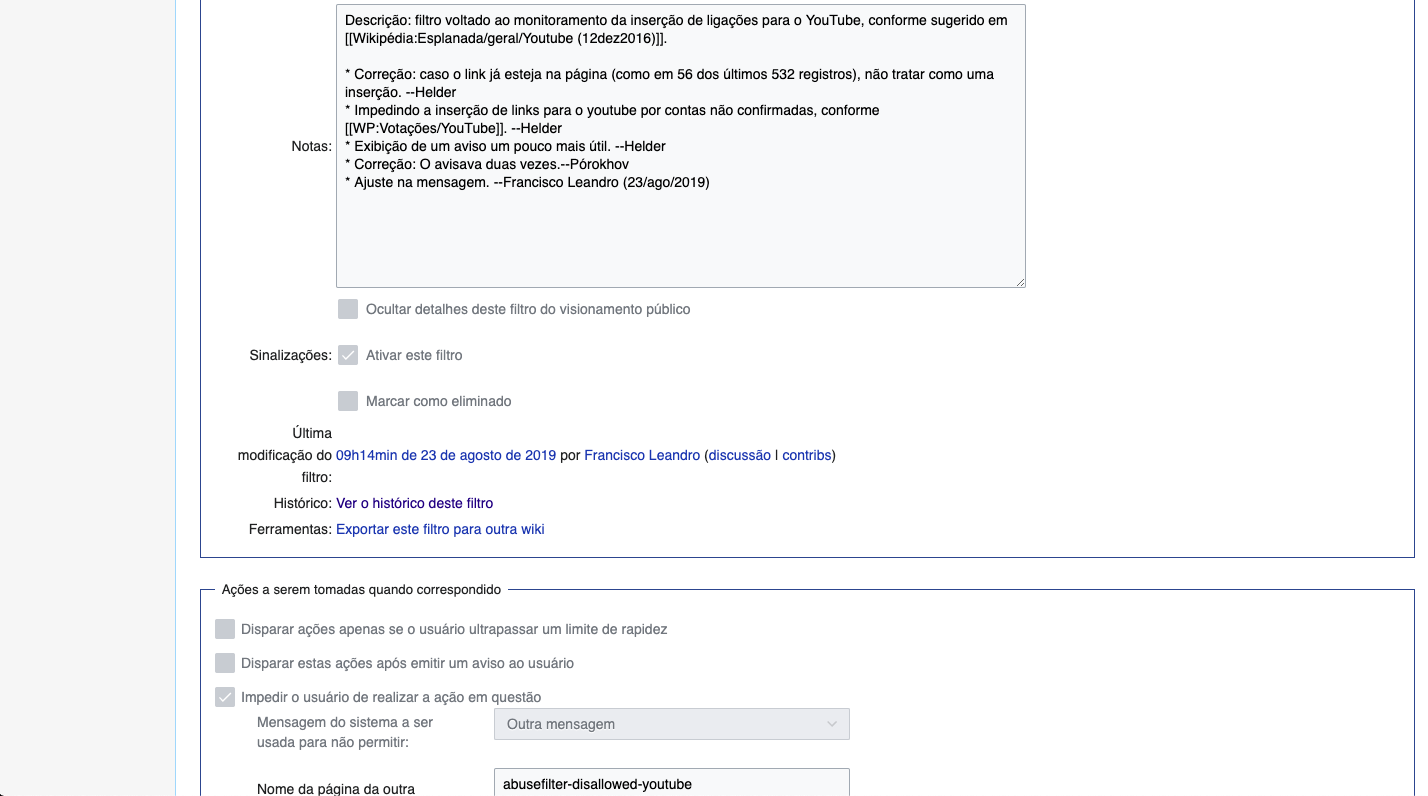
\includegraphics[width=1\textwidth]{Images/pagina_edicao_administadores.png}
    \caption{Continuação da página exibida na figura anterior, com mais opções de configurações dos filtros visíveis \citewiki{ptwiki_editar_filtros_1_edicao}.}
    \label{fig:pagina_edicao_administradores}
\end{figure}

Além das páginas especiais, existe uma página wiki ``comum'', que pode ser editada como as outras, que versa sobre os filtros de edição, explicando seu funcionamento. \footnote{Página disponível em https://pt.wikipedia.org/wiki/Wikipédia:Filtro\_de\_edições .} Assim como toda página wiki convencional, ela é acompanhada de uma página de discussão onde editores podem abrir tópicos para debater seu conteúdo.

Porém, esta página aparenta não contar com a atenção dos wikipedistas. Desde 2019 foram abertos 20 novos tópicos de discussão nela por usuários novatos mas, decorridos 8 meses do ano de 2020, apenas um havia recebido resposta de um editor experiente, com os demais 19 tópicos seguindo visíveis e ignorados. \citewiki{ptwiki_filtro_de_edicoes}

Até o final de 2019 existia uma outra página wiki, chamada ``Filtro de Edições/Solicitações'', que concentrava pedidos para alterações nos filtros. Nela podemos ainda encontrar assustadores 125 novos tópicos sobre o funcionamento dos filtros de edições que foram criados e não obtiveram nenhuma resposta. \citewiki{ptwiki_filtros_edicao_solicitacoes}

Durante um certo período de tempo, esta página recebia um volume de acessos maior de novatos, pois o aviso de ``desautorizar'' apresenta um link para ela com a seguinte mensagem \textit{``Se você crê que a sua edição foi construtiva, por favor informe-nos o que você estava a tentar fazer. Nós vamos analisar o problema e informar a causa, ou vamos corrigir o sistema para que tal mensagem não apareça novamente, se for necessário.''} \citewiki{ptwiki_mediawiki_abusefilter_disallowed}. Porém, desde o dia 1 de dezembro de 2019, quando foi aprovada uma proposta de fusão de diversas páginas de contato da Wikipédia em português \citewiki{ptwiki_esplanada_geral_duvidas-fale}, a mensagem de ``desautorizar'' dos filtros passou a linkar os usuários para a página ``Wikipédia:Tire Suas dúvidas''\citewiki{ptwiki_ajuda_duvidas}. Por ser esta uma página mais genérica onde são tratados diversos assuntos, não nos foi possível observar o volume de mensagens relativos a filtros que chegam até ela, mas cabe destacar que este novo destino é monitorado por mais wikipedistas, e são raros os novos tópicos abertos por lá que ficam sem resposta.

% aqui tem uma pequena mudança, vinhamos falando de onde os novatos são encaminhados, agora seguimos o rastro "mais pra dentro", buscando debates avançados

Seguimos buscando rastros de debates sobre os filtros, e adentramos o ``Café dos administradores'', uma página wiki que pode ser lida por todos mas somente pode ser editada por usuários com permissão de administrador. Voltando o histórico da página até o início de 2018, encontramos apenas uma menção ao filtro de edições, onde um administrador solicita ajuda de alguém \textit{``familiarizado com o assunto''} para implementar em filtro um bloqueio parcial a um usuário que fora decidido em uma votação. Em menos de 12 horas, o pedido foi respondido como um direto \textit{``feito''}, e nunca mais o filtro de edições fora mencionado no café dos administradores. \citewiki{ptwiki_diferenca_edicao_cafe-administradores}

% outra mudança no texto. indo atrás de depoimentos

Em meio a tão poucos debate e discussões, aceitamos então que seguir o rastro digital da criação dos filtros não estava apresentando muitos resultados para nossa pesquisa. Decidimos assim partir para o campo e conversamos com administradores da Wikipédia em português mais engajados na tarefa de criar, manter e atualizar filtros.

OTAVIO1981, ou simplesmente Otávio, é um usuário ativo da Wikipédia desde 2007. Com mais de 36 mil edições\citewiki{ptwiki_edicoes_grupos_otavio1981}, em março de 2015, ele que já havia sido administrador entre 2013\citewiki{ptwiki_administradores_pedido_otavio1981/1} e 2014\citewiki{enwiki_wikimedia_steward_resquest_permissions}, se propõe à assumir a posição novamente, dizendo explicitamente em seu pedido de aprovação que \textit{``firmo o compromisso de orientar e seguir com a atualização dos filtros de edição, etiquetas, e atualizações no mediawiki''} \citewiki{ptwiki_administradores_pedido_otavio1981}

Otávio, que não trabalha na área de computação, resolveu \textit{``estudar e aprender como fazer  expressões regulares para atuar com os filtros.''}\footnote{Até que seja indicado o contrário, todas as citações que seguem são retiradas da entrevista realizada com OTAVIO1981}, e se propôs a ser um voluntário que atua ativamente na melhoria desta ferramenta e na orientação a usuários que interajam com ela. Em sua candidatura a administrador em 2013, Otávio afirmou que desejava ter acesso administrativo pois \textit{``entendo que o acesso é prioritariamente para atuar na área de filtros que não possui instalado aqui outro estatuto que permita acesso as ferramentas necessárias''}.

Em outras palavras, como apenas administradores podem acessar as ferramentas completas dos filtros de edição, ele precisava ser um administrador da Wikipédia em português para seguir com suas contribuições nesta area\citewiki{ptwiki_administradores_pedido_otavio1981/1}. Novamente, em seu questionário de renomeação em 2015, o editor foi enfático ao afirmar que \textit{``O filtro de edições possui alguns recursos que estão disponíveis somente para administradores, assim como filtros que são privados, portanto não é possível orientar a atualização para terceiros sem acesso a estes recursos''}. Assim como em 2013, o novo pedido de Otávio para se tornar administrador é aprovado sem nenhum voto contrário.

% aqui teve uma apresentacao do Otavio virando admin para poder mexer nos filtros, para baixo entra já numa explicao da criacao dos filtros, que estavamos procurando

Otávio nos conta que houveram três grandes \textit{``ondas de atividade''} na construção e melhoria de filtros na Wikipédia em português, em momentos que alguns voluntários se dedicaram mais intensamente a melhorá-los. Houve uma primeira onda inicial quando os filtros foram implementados entre 2009 e 2010, uma segunda onda em 2013, da qual ele participou ativamente, e depois uma terceira onda em 2017. 

\begin{figure}[H]
    \centering
    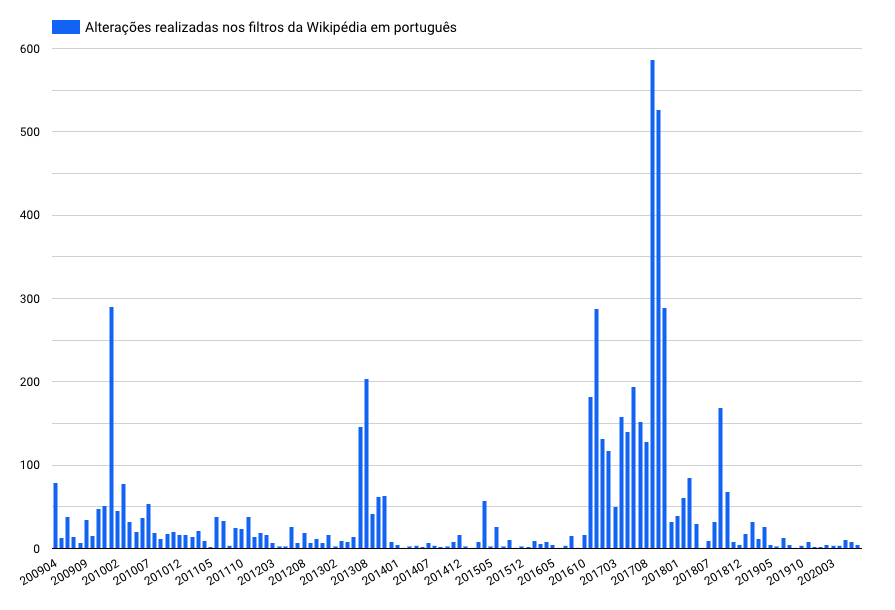
\includegraphics[width=1\textwidth]{Images/grafico_alteracoes_filtros.png}
    \caption{Volume de alterações nos filtros da Wikipédia em português por mês. (fonte: https://datastudio.google.com/u/0/reporting/6b38f843-1507-4364-85e9-bdef43296881/page/TRabB ).}
    \label{fig:grafico_alteracoes_filtros}
\end{figure}

Otávio esteve muito ativo na onda de interesse pelos filtros em 2013, que aconteceu devido a polêmica retirada do modo emergencial do CAPTCHA \footnote{Esta polêmica será detalhada mais a frente no texto.}. Esta ação fez o número de edições na Wikipédia em português subir e levou a comunidade a buscar novas formas de automatizar o combate a edições ruins.

O usuário explica que nesta segunda onda, \textit{``apesar de não terem conseguido chegar em uma \textbf{formalidade científica} para validar se um filtro estava dando resultado''} (grifo nosso), criaram critérios para testar os filtros e decidir se eles seriam \textit{``promovidos''}.

Neste processo foi realizada uma força tarefa para avaliar cada disparo dos filtros, apontando se fora um ``verdadeiro positivo'' ou um ``falso positivo''. Assim, para cada filtro foi criada uma página wiki onde o resultado da avaliação de todas as suas ações deveria ser publicado \footnote{Um exemplo de página de avaliação dos filtros pode ser encontrado em: https://pt.wikipedia.org/wiki/Wikipédia:Filtro\_de\_edições/An\%C3\%A1lise/Filtro\_70}. Visando facilitar não só o trabalho de avaliação dos disparos dos filtros como também a futura agregação e comparação dos dados gerados, o usuário He7d3r criou um script \footnote{Disponível em meta.wikimedia.org/w/index.php?title=User:He7d3r/Tools/AbuseLogStatus.js} para automatizar a geração destas avaliações de forma rápida e padronizada.

Foram realizadas aproximadamente 7 mil avaliações das ações dos filtros e, apesar de toda a comunidade ter sido convidada a colaborar, mais de 92\% das ações foram realizadas por apenas 3 usuários (OTAVIO1981, Rjclaudio e He7d3r), sendo OTAVIO1981 sozinho responsável por mais da metade delas. Vale mencionar que sempre que um usuário anotava que uma edição fora um ``falso positivo'', ele era convidado a escrever um comentário sobre sua avaliação, e estes comentários posteriormente seriam utilizados para buscar realizar melhorias nos filtros.

\begin{figure}[H]
    \centering
    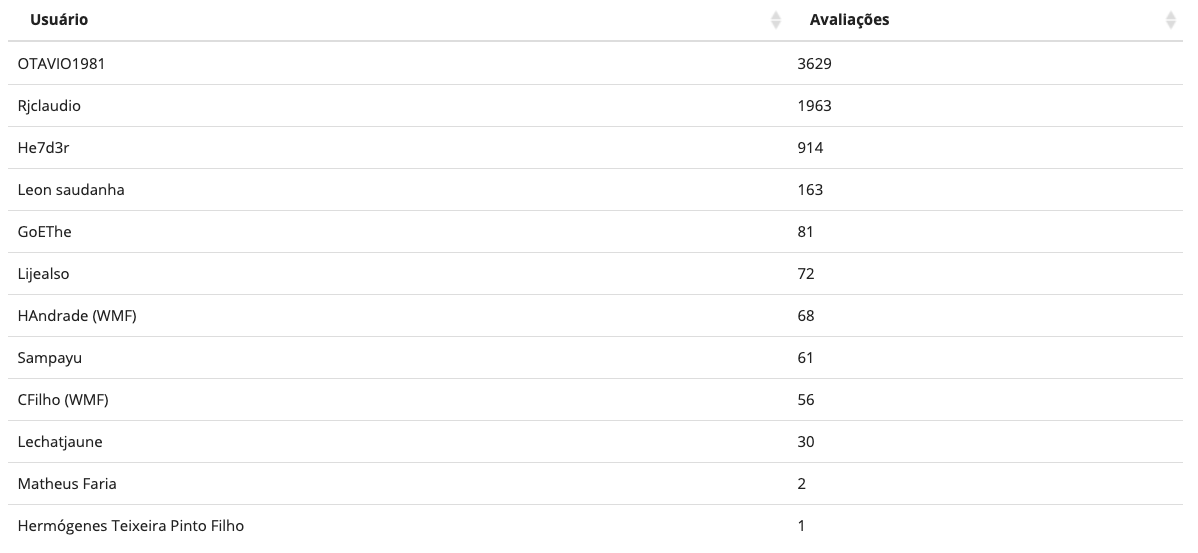
\includegraphics[width=1\textwidth]{Images/pagina_analise_filtros.png}
    \caption{Edições feitas nas páginas de Análise dos Filtros (\cite{quarry_users_evaluating_filters}).}
    \label{fig:pagina_analise_filtros}
\end{figure}

Não por acaso, estes mesmo três usuários mais ativos na avaliação dos filtros foram também os mais ativos na edição dos mesmos durante a chamada segunda onda. Entre julho e novembro de 2013, Rjclaudio realizou 286 alterações nos filtros, seguido por He7d3r com 139 e Otávio com 51.

Durante os esforços da segunda onda, os usuários mais engajados na melhoria dos filtros debatiam em um espaço público\citewiki{ptwiki_discussao_filtro_edicao_analise} os resultados encontrados e coordenavam ali as alterações que seriam feitas. Os índices de acertos e erros de cada filtro avaliado passaram a ser consolidados em uma página, disponível até hoje no endereço https://pt.wikipedia.org/wiki/Wikipédia:Filtro\_de\_edições/Análise. 

Nestas páginas de análise, foi possível observar que vários filtros apresentavam um volume consideravelmente alto de erros, de onde podemos destacar os já citados filtros 113 e 70, que são os mais ativos na Wikipédia em português na ação de ``desautorizar'' uma edição. Para nossa surpresa, observamos que das 112 ações do filtro 113 avaliadas pela força tarefa, 31,3\% foram consideradas falsos positivos e, com um espaço amostral maior, com 570 edições avaliadas, o filtro 70 aparenta ter sido disparado indevidamente 22,8\% das vezes.

Estes grandiosos números aparentavam anunciar um cenário trágico, mas ao analisarmos o histórico de edições destes filtros podemos entender melhor o que estava acontecendo. Seguindo o que Otávio chama de \textbf{\textit{``uma busca por formalidade científica''}}, os filtros estavam sendo criados somente com ações de etiquetar, para serem testados na vida real, avaliados, melhorados, e apenas passariam a performar ações mais drásticas quando apresentassem resultados considerados satisfatórios.

Ao olharmos o caso de filtro 113, por exemplo, identificamos 13 edições nele durante a segunda onda\citewiki{ptwiki_filtro_abuso_historico113} antes que fosse chamado a realizar qualquer ação que interferisse no curso dos usuários. Após diversas revisões iniciais, o filtro passa para fases de testes, onde são intercaladas as ações de “etiquetar”, “avisar” e “desautorizar”, se estabilizando ao final da onda, em novembro de 2013, como um filtro que “apenas” etiqueta.

Em abril de 2014 ele viria a ser novamente alterado para se tornar um filtro que também “avisa”, voltando a ser um “desautorizador” apenas em março de 2018, após uma proposta aprovada na Esplanada \citewiki{ptwiki_esplanada_geral_verificabilidade_artigos}.

A proposta acima, após uma breve discussão que contou com o apoio de quatro usuários e nenhuma objção, foi implementada pelo usuário “Silent!”. Ele que, desde sua nomeação para administrador em 2016, se tornou o usuário mais ativo da história da Wikipédia em português nos filtros de edição. Silent, um programador de carreira, nos conta \footnote{Até que seja indicado o contrário, todas as citações que seguem são retiradas da entrevista realizada com ``Silent!''.} que após se tornar administrador da Wikipédia em português percebeu que existia uma defasagem nos filtros, que não eram atualizados há um tempo, e passou a se dedicar intensamente a esta tarefa.

Sua determinação cria então o que chamamos de “terceira onda” de filtros na Wikipédia em português, que começa em novembro de 2016 e vai até novembro de 2017. Durante ela, Silent é responsável por 2675 edições nos filtros, respondendo assim por mais de 90\% das ações ali realizadas no período.

O usuário nos conta que \textit{“a alta defasagem dos filtros me levou a criar e adaptar muita coisa que já existia para se atualizar aos problemas de vandalismo da época. Para se ter uma noção, os filtros não barravam diversos xingamentos extremamente nocivos em português de Portugal, como “pila” e “cona”, que são palavrão que remetem ao órgão sexual masculino e feminino, respectivamente; ou seja, eles retratavam uma visão muito mais brasileira da coisa, deixando de lado ofensas em português europeu”}.

Em seu processo de melhoria dos filtros ele lamenta que a ferramenta não permita exibir um \textit{feedback} maior para os usuários que estão adicionando conteúdo considerado problemático: \textit{“não é possível exibir, naquele aviso que aparece após uma edição ser bloqueada por um filtro, qual é expressão que gerou o bloqueio”}, e também nos conta que a página para onde outrora os usuários eram encaminhados cumpria um papel importante no trabalho de adequação dos filtros para diminuir os falsos-positivos. \textit{“Foi por ali [Página Wikipédia:Filtro de edições/Solicitações] que eu fiquei sabendo de vários falsos-positivos gerados em modificações feitas por mim nos filtros.}”

Perguntado sobre a necessidade de encaminhar propostas de alterações nos filtros para a comunidade, o usuário nos explica que \textit{“na realidade não há um local específico para o debate de alterações nos filtros e nem há uma necessidade de que cada novo filtro seja implantado via consenso. Todas àquelas alterações feitas por mim, principalmente no fim de 2016 e por todo ano de 2017, foram feitas de forma unilateral”}, complementando que seu processo de controle de qualidade dos mesmos é feito de forma artesanal: \textit{“da minha parte, são todos testados individualmente e de forma manual, disparo por disparo a fim de identificar problemas ou oportunidades de melhoria. Não há uma página específica, mas há uma ferramenta que contabiliza o índice de disparos”}.

%aqui dou uma desviada para falar do ptwikis

A citada ferramenta é parte do projeto PTWIKIS, e fora criada pela comunidade lusófona, com especial liderança do usuário danilo.mac, durante a segunda onda de filtros. O “ptwikis” é um projeto de criação de ferramentas de visualização de dados que exibe gráficos rápidos para uma série de informações sobre as Wikipédias, \textit{“criado para concentrar em um único projeto ferramentas que sejam de interesse dos projetos lusófonos e para incentivar a cooperação entre usuários para o desenvolvimento dessas ferramentas”}. \citewiki{ptwiki_ptwikis}

Apesar de inicialmente criada pela e para a Wikipédia em português, hoje a ferramenta apresenta opções para seus dados serem gerados sobre qualquer wiki dentro do movimento Wikimedia, e também é utilizada por editores de outros projetos e idiomas. Em sua seção dedicada ao monitoramento de filtros, a ferramenta exibe duas telas, uma com todos os filtros e suas ações totalizadas nos últimos 30 dias \citewiki{ptwiki_acoes_filtros} e  outra com uma linha do tempo, exibindo as ações dos filtros selecionados totalizadas por dia \citewiki{ptwiki_acoes_filtros_exemplo3_7}.

O projeto ptwikis fora criado não coincidentemente em julho de 2013, exatamente quando se iniciava a segunda onda de melhoria dos filtros. A remoção do modo emergencial do CAPTCHA acontecida no início daquele ano aparenta ter gerado um grande efeito na comunidade da Wikipédia em português, que passou a buscar conhecer melhor suas dinâmicas e ferramentas. Para compreendermos o que aconteceu no referido evento e entendermos o tamanho de sua influência na comunidade, exploraremos o funcionamento da ferramenta de CAPTCHA na próxima seção.

\subsection{CAPTCHA}

CAPTCHA, sigla em inglês para \textit{``Completely Automated Public Turing test to tell Computers and Humans Apart''} \footnote{Em tradução livre: \textit{“teste de Turing público completamente automatizado para diferenciação entre computadores e humanos”.}}, é uma ferramenta muito comum na internet para tentar evitar ações automatizadas realizadas por \textit{``robôs mal intencionados''}. \citewiki{ptwiki_captcha_definicao}

Na Wikipédia, o captcha se materializa em forma de palavras em inglês onduladas e picotadas, em um padrão que seus desenvolvedores esperam ser muito complicado para robôs entenderem, mas simples para humanos. \citewiki{ptwiki_captcha_definicao}

\begin{figure}[H]
    \centering
    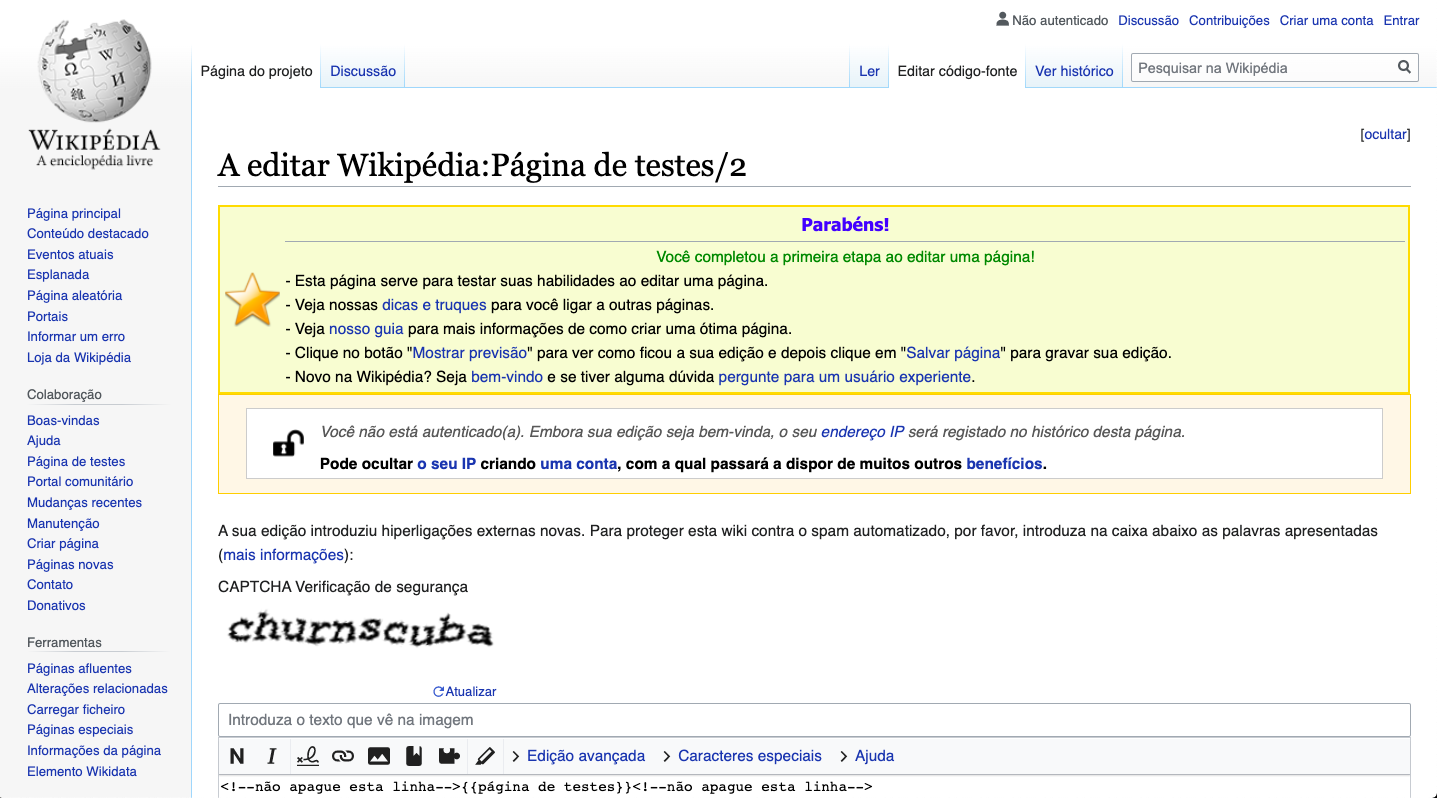
\includegraphics[width=1\textwidth]{Images/mediawiki_solicita_captcha.png}
    \caption{MediaWiki solicitando que um usuário anônimo resolva um captcha para salvar sua edição. Detalhe para a caixa de \textit{“parabéns por sua primeira edição feita”} erroneamente sendo exibida em destaque, mesmo com a edição não tendo ainda de fato sido salva.}
    \label{fig:mediawiki_solicita_captcha}
\end{figure}

O teste é implementado pela \textit{ConfirmEdit}, uma extensão feita para o MediaWiki que, desde a versão 1.18 do software, já é distribuída com ele por padrão. Segundo o \textit{Wikiapiary}, hoje essa ferramenta de CAPTCHA para MediaWiki é utilizada por aproximadamente 10 mil wikis diferentes pelo mundo\citep{extension_confirm_edit}.

Tanto a página oficial da extensão\citewiki{enwiki_extension_confirm_edit} como a página na Wikipédia em português sobre a ferramenta \citewiki{ptwiki_captcha_definicao} afirmam que ela é utilizada para coibir spambots, \textit{“que, através de contas anônimas, provocam vandalismo em diversos artigos em um curto espaço de tempo”}. Visando alcançar este objetivo, atualmente a configuração padrão do CAPTCHA nas Wikipédias dita que ele deve aparecer sempre que um usuário anônimo ou não confirmado (também chamado de novato) fizer uma edição adicionando um link externo.

A expectativa anunciada pelos wikipedistas é que humanos consigam facilmente resolver o teste, e apenas os scripts maliciosos sejam barrados pela ferramenta. Porém, a realidade não se mostra tão óbvia. Na própria página sobre a ferramenta existem três notas de rodapé apontando para transbordamentos da atuação do captcha: [1] o fato das palavras serem em inglês aumenta a dificuldade de compreensão de não falantes deste idioma, [2] usuários cegos não tem chances de resolver este captcha, que é totalmente dependente da visão e [3] quando ativado o modo emergencial, todas as edições feitas por anônimos e novatos, adicionando ou não links externos, precisam resolver o captcha. \citewiki{ptwiki_captcha_definicao}

Das três controvérsias listadas pelos wikipedistas sobre o captcha decidimos em nossa pesquisa seguir a terceira, pois fora exatamente a desativação deste modo emergencial em 2013 que desencadeara a segunda onda de filtros trabalhada na seção anterior.

% aqui acaba uma introdução ao captcha e começa a controvérsia

No dia 8 de abril de 2013, o usuário Helder.wiki cria um tópico na página ``Esplanada/anúncios'', o fórum central de notícias internas da Wikipédia em português, intitulado \textit{``Remoção do modo emergencial do CAPTCHA''}, e seu conteúdo tem apenas o texto \textit{``Ver gerrit:58081''}, com um link para um ticket no sistema de revisão de scripts dos servidores do Movimento Wikimedia, onde o código da anunciada alteração havia sido aprovado para ser executado nos servidores da Wikipédia em português. Este acontecimento desperta revolta em vários membros da comunidade lusófona e controvérsias tanto sobre a governança da comunidade como sobre o controle de qualidade dos verbetes se acaloram. \citewiki{ptwiki_esplanada_geral_remocao_modo_captcha}

É interessante notar que o uso do modo emergencial do CAPTCHA havia sido deslocado pela comunidade lusófona. Enquanto originalmente pensada e documenta para ser utilizada contra robôs maliciosos, a ferramenta passou a ser vista pela Wikipédia em português como uma ajudante na diminuição do volume de edições potencialmente ruins que precisariam ser revisadas por humanos.

A discussão na Esplanada então segue com mensagens em português, inglês e italiano, pois fora um usuário nativo deste idioma que encaminhara a desativação do modo emergencial, após o mesmo  ter sido notado \textit{“esquecido ativo”}, após ter sido ligado durante um ataque de robôs spammers no longíquo janeiro de 2008\citewiki{ptwiki_esplanada_arquivo_2008janeiro}.

Sentindo ter sua autonomia ferida, vários membros da comunidade lusófona acusam a \textit{“comunidade técnica de administradores de servidores”} de ingerência, e partem para travar o debate em outros espaços do movimento Wikimedia. Assim, locais como o Bugzilla (hoje rebatizado Phabricator) \citep{remove_ptwiki_ptwikinews_captcha_mode} e até mesmo o Gerrit \citewiki{remove_ptwiki_ptwikinews_captcha_mode_gerrit}, sempre vistos como \textit{``espaços técnicos''}, onde são discutidas apenas formas de fazer o software funcionar, e não as decisões das comunidades, acabam se tornando palco de discussões e acusações sobre governança dos projetos, definições de consensos e esforços de combate ao vandalismo.  

Aproximadamente 24 horas após o anúncio feito por Helder.wiki na Esplanada, a mudança estava efetivada e o modo emergencial do captcha removido da Wikipédia em português. O usuário Rjclaudio então propõe que pesquisas sejam feitas para medir mudanças de comportamento e testar na prática se os cenários apocalípticos decorrentes desta mudança de configura/cão, alardeados por alguns usuários no acalorado debate, se tornariam realidade. Assim, vemos a emergência de centrais de cálculo da comunidade e esforços para criação de métricas que traduzam as “percepções subjetivas” sentidas pelos usuários em “números objetivos”. Observamos então a tentativa de estabilização de traduções. Dois grupos diferentes buscam fazer inferências e convencer o movimento que a sua leitura seria a forma certa de interpretar os dados, com os mesmos números servindo de base tanto para teses de que a desativação do modo emergencial do CAPTCHA havia sido benéfica, tanto como para a interpretação de que essa ação estaria matando o projeto. Temos então colocada uma disputa entre duas realidades diferentes, que por serem contraditórias e disputarem o mesmo espaço de poder, precisam provar como falsa a tese adversária para poder sair vitoriosa da peleja e então nortear as ações a serem tomadas em seguida.

É interessante notar a riqueza de desdobramentos que uma pane pode causar. Diversas iniciativas são tomadas para criar novas composições estáveis para a manutenção e continuidade do projeto, e uma vez aberta a caixa-preta das edições represadas pelo modo Emergencial do Captcha não será mais satisfatório e suficiente simplesmente o ativar novamente para encerrar a controvérsia. Agora existe uma boa parcela de usuários genuinamente preocupados e engajados em entender quais edições que outrora estavam represadas por essa configuração agora estão sendo feitas, e qual o perfil de usuários que as estão fazendo. 

Com isso, as barreiras automatizadas para edições implementadas no MediaWiki passam a ser vistas como um ponto de passagem obrigatório no debate sobre o crescimento da comunidade e a recepção de novos usuários, e algumas destas barreiras implementadas em software passarão então a receber atenção e ser dissecadas por alguns usuários mais dedicados ao assunto.


Em meio diversas visões de mundo, disputas e acusações, a comunidade lusófona parece se aproximar de um consenso sobre a tão polêmica configuração, que arriscamos resumir em ``O modo emergencial do CAPTCHA ajuda no controle de qualidade ao diminuir o volume de edições, mas queremos controlar a qualidade de outra forma que não tornando a vida de quem quer editar mais difícil'' \footnote{Para mais detalhes sobre esta controvérsia ver https://pt.wikipedia.org/wiki/Wikipédia\_Discuss\%C3\%A3o:Captcha\#Apanhado\_de\_discuss\%C3\%B5es\_sobre\_o\_CAPTCHA\_para\_registo}. 

Em um movimento de construção de novas formas de combate às edições consideradas ruins, que não passasse simplesmente por dificultar a vida dos usuários novatos, a Wikipédia em português assiste então ao renascimento do ``Projeto Antivandalismo'', que apesar de existir desde 2008, estava praticamente inativo por anos e passa a receber diversas contribuições ao longo do ano de 2013.

\begin{table}
\centering
\begin{tabular}{c|c}\hline
 \textbf{Ano} & \textbf{Edições}\\ \hline
    2017 & 2\\\hline
    2016 & 10\\\hline
    2015 & 6\\\hline
    2014 & 24\\\hline
    2013 & 364\\\hline
    2012 & 2\\\hline
    2011 & 0\\\hline
    2010 & 7\\\hline
    2009 & 13\\\hline
    2008 & 27\\\hline
\end{tabular}
\caption{Total de edições por ano na página Wikipédia Discussão:Projetos/AntiVandalismo.\citep{quarry_edits_page_year}}
\label{tab_edicao_wiki_antivandalismo}
\end{table}

Em paralelo, enquanto busca criar alternativas futuras de controle de qualidade,  a comunidade lusófona solicita a intervenção da WMF na ``crise diplomática'' instaurada dentro do movimento Wikimedia, pedindo que sua autonomia seja respeitada pela ``comunidade do MediaWiki'', e que o modo emergencial do CAPTCHA seja reativado. O pedido deixa claro não haver um ``argumento técnico'' para comprovar ataques de robôs, e deixa explícito seu intuito de diminuir o volume de edições feitas por novatos. A fundação então responde que esta não é a função da ferramenta, mas que, por ela ter sido esquecida ativada por tanto tempo, iria então permitir temporariamente sua reativação até o final de 2013, reforçando que o combate a edições ruins deveria a partir de então ser feito por outros meios, como os que estavam sendo discutidos no \textit{``Projeto Antivandalismo''}.  \citewiki{ptwiki_discussao_captcha}

Desta forma, diversos usuários se engajam em projetos tanto para freiar automaticamente edições não desejadas (criando a segunda onda de atualização dos filtros), como para desenvolver ferramentas de análise e monitoramento de metadados de comportamento na comunidade (criando o já citado projeto “ptwikis”), como também para melhorar a recepção de novatos bem intencionados (iniciativas que serão citadas no próximo capítulo). Assim, com a comunidade engajada em diversas novas formas de combate ao vandalismo e a melhoria na recepção de novatos, ao se iniciar o ano de 2014, o modo emergencial do CAPTCHA é finalmente desativado sem maiores controvérsias.

%aqui acaba a treta de 2013 e começo a falar de como essa ferramenta é monitorada hoje

Passados seis anos da contenda e da reestabilização do CAPTCHA como uma ferramenta que deve apenas combater \textit{“robôs spammers maliciosos”} e não usuários inexperientes, buscamos saber como a comunidade da Wikipédia em português monitora o funcionamento da ferramenta.

Começamos nossa busca pelas páginas dentro da Wikipédia sobre a ferramenta do captcha, mas encontramos apenas textos informativos. A página de discussão da ferramenta, bastante acalorada no passado, não recebe nenhuma contribuição desde julho de 2013.

Não encontrando indícios de monitoramento e atividade da ferramenta pelas páginas wiki, resolvemos buscar informações com os usuários mais engajados nos filtros com quem conversamos. Apesar das ferramentas serem próximas e terem funcionalidades parecidas, tanto Otávio como Silent, que são engajados no acompanhamento dos filtros, não souberam responder onde e/ou se existe um log com as edições barradas pelo CAPTCHA, e desconhecem a possibilidade de se realizar uma auditoria em seu funcionamento. 

Buscamos então o maior fórum público da Wikipédia em português: a Esplanada. A Esplanada é um conjunto de páginas dentro da Wikipédia onde usuários podem fazer comentários, propostas, tirar dúvidas, etc. Como explicado por ela mesma, as páginas da Esplanada “servem para todo o género de conversas e perguntas sobre a Wikipédia lusófona.” \citewiki{ptwiki_esplanada}

Criamos então um novo tópico na Esplanada perguntando para a comunidade onde poderiam ser encontrados os logs de ação do captcha. \citewiki{ptwiki_esplanada_geral_registro_captcha_spam_blacklist}  O tópico recebeu dois comentários, dos usuários danilo.mac e ALBERTOLEONCIO, com ambos informando desconhecer qualquer tipo de registro relacionado às ações do CAPTCHA na Wikipédia.

Por fim, buscamos apoio na página de discussão oficial da extensão responsável pelo CAPTCHA, na wiki mediawiki.org . Lá, passado um ano da publicação de nossa pergunta sobre onde encontrar logs das ações do CAPTCHA em uma Wikipédia, nosso tópico continua sem ter recebido um comentário sequer de outro usuário. \citewiki{enwiki_log_captcha_extension_talk_confirmedit}

Gostaríamos de ter avançado em nossa investigação respondendo perguntas como ``qual o percentual de acerto/erro dos usuários que respondem ao CAPTCHA?'', “quais URLs estão sendo adicionadas por tentativas bloqueadas?” e “quais páginas estão sendo editadas por usuários que se deparam com o CAPTCHA?”. Porém, a falta de dados estruturados coletados nos deixou em um beco sem saída, com a certeza de que nenhum humano em toda comunidade teria a capacidade de responder a tais questionamentos.

Encerramos então por aqui nossa busca por mais informações sobre a atividade desta ferramenta automatizada, com a convicção de que ela hoje opera como uma caixa-preta invisível na Wikipédia em português, contando o MediaWiki com a mais alta confiança da comunidade para a implementar e barrar edições, não sendo objeto de nenhum tipo de verificação ou auditoria de suas ações.